
\documentclass[12pt,letterpaper]{article}


\usepackage[top=1in, 
		    bottom=1in,
		    left=1in,
		    right=1in]{geometry}
\usepackage{setspace}	% makes the \singlespacing, \onehalfspacing, and \doublespacing commands available
% \usepackage[en-US]{datetime2}
% \DTMlangsetup{showdayofmonth=false}
% \usepackage{titlesec}
\usepackage{listings}	% allows for placing programming code to be displayed correctly
\usepackage{siunitx}	% units
\usepackage{amsmath}
\usepackage{amsfonts}
\usepackage{amssymb}
\usepackage{graphicx}
\usepackage{booktabs}
\usepackage{multirow}
\usepackage{pgfplots}
\pgfplotsset{compat=newest}
\usepackage{tikz}
%\usetikzlibrary{shapes.geometric}
% \usepgfplotslibrary{external} 
% \tikzexternalize[prefix=pdfimages/,
% 		        mode=list and make]
\usepackage{caption}
\usepackage[list=true,
		     listformat=simple]{subcaption}
%\usepackage{cleveref}	% this should really go last
% \usepackage[colorlinks,
% 		     linkcolor=black,
% 		     citecolor=black,
% 		     plainpages=false,
% 		     pdfpagelabels]{hyperref}
% \usepackage[all]{hypcap}
\usepackage{cleveref}
% \doublespacing

\pagenumbering{gobble}
\newcommand{\mymder}[2]{\ensuremath{\frac{\mathrm{D}#1}{\mathrm{D}#2}}}
\newcommand{\mypder}[2]{\ensuremath{\frac{\partial #1}{\partial #2}}}
\newcommand{\mypdertwo}[2]{\ensuremath{\frac{\partial^2 #1}{\partial #2^2}}}
\newcommand{\mymdervec}[1]{\ensuremath{mypder{#1}{t} + }}
\newcommand{\myder}[2]{\ensuremath{\frac{d#1}{d#2}}}
\newcommand{\mydiv}[1]{\ensuremath{\nabla \cdot {#1}}}
\newcommand{\myfrac}[2]{\ensuremath{^{#1}\!/_{#2}}}
\newcommand{\myfunc}[2]{\ensuremath{#1 \left( #2 \right)}}
\newcommand{\myparen}[1]{\ensuremath{\left( #1 \right)}}
\newcommand{\mybrack}[1]{\ensuremath{\left[ #1 \right]}}
\newcommand{\mybrace}[1]{\ensuremath{\left\{ #1 \right\}}}
\newcommand{\mysin}[1]{\ensuremath{\myfunc{\mathrm{sin}}{#1}}}
\newcommand{\mycos}[1]{\ensuremath{\myfunc{\mathrm{cos}}{#1}}}
\newcommand{\myexp}[1]{\ensuremath{\myfunc{\mathrm{exp}}{#1}}}
\newcommand{\myint}[4]{\ensuremath{\int_{#1}^{#2} {#3} d {#4}}}


\newcommand{\Rld}{\ensuremath{\mathit{Re}}}
\newcommand{\St}{\ensuremath{\mathit{St}}}
\newcommand{\Prn}{\ensuremath{\mathit{Pr}}}
\newcommand{\Sc}{\ensuremath{\mathit{Sc}}}
\newcommand{\Sh}{\ensuremath{\mathit{Sh}}}
\newcommand{\Nu}{\ensuremath{\mathit{Nu}}}
\newcommand{\Bi}{\ensuremath{\mathit{Bi}}}


\let\textacute\'
\let\textgrave\`


\newcommand{\includetikz}[2]{%
    \tikzsetnextfilename{#2}%
    \input{#1#2.tex}%
}

\begin{document}

\noindent
MECH 131A Homework 6

\noindent
Assigned date: November $29^{\mathrm{th}}$, 2024

\noindent
Due date: December $12^{\mathrm{th}}$, 2024

\subsubsection*{Instructions}
\begin{enumerate}
	\item Indicate the names of your study group members.
	\item Draw a sketch of the problem.
	\item If using a specific solution methodology is specified, please include a copy of the Python/MATLAB script.
		Some sort of package that calculates properties, such as CoolProp, will likely be very useful. 
	\item If using a specific solution methodology is \textit{not} specified, please include a copy of your computational methodology.
\end{enumerate}


\subsubsection*{Problem Set}
\begin{enumerate}
    \item A \SI{0.6}{\milli\meter} diameter wire, with $\epsilon = 0.85$, is drawn out through a mandril at \SI{950}{\celsius}.
        The wire then passes through a long cylindrical shield of commercial aluminum sheet, \SI{7}{\centi\meter} in diameter.
        The shield is horizontal in still air at \SI{25}{\celsius}.
        What is the temperature of the shield?
        Is it reasonable to neglect natural convection inside the or radiation outside the shield?

    \item Consider the three-surface enclosure shown.
        The lower plate ($A_1$) is a black disk of \SI{200}{\milli\meter} diameter and is supplied with a heat rate of \SI{10000}{\watt}.
        The upper plate ($A_2$), a disk coaxial to $A_1$, is a diffuse, gray surface with $\epsilon = 0.8$ and is maintained at $T_2 = \SI{473}{\kelvin}$.
        The diffuse, gray sides between the plates are perfectly insulated. Assume convection heat transfer is negligible.
        Determine the operating temperature of the lower plate T1 and the temperature of the insulated side T3.
    
    \begin{figure}[!htpb]
        \centering
        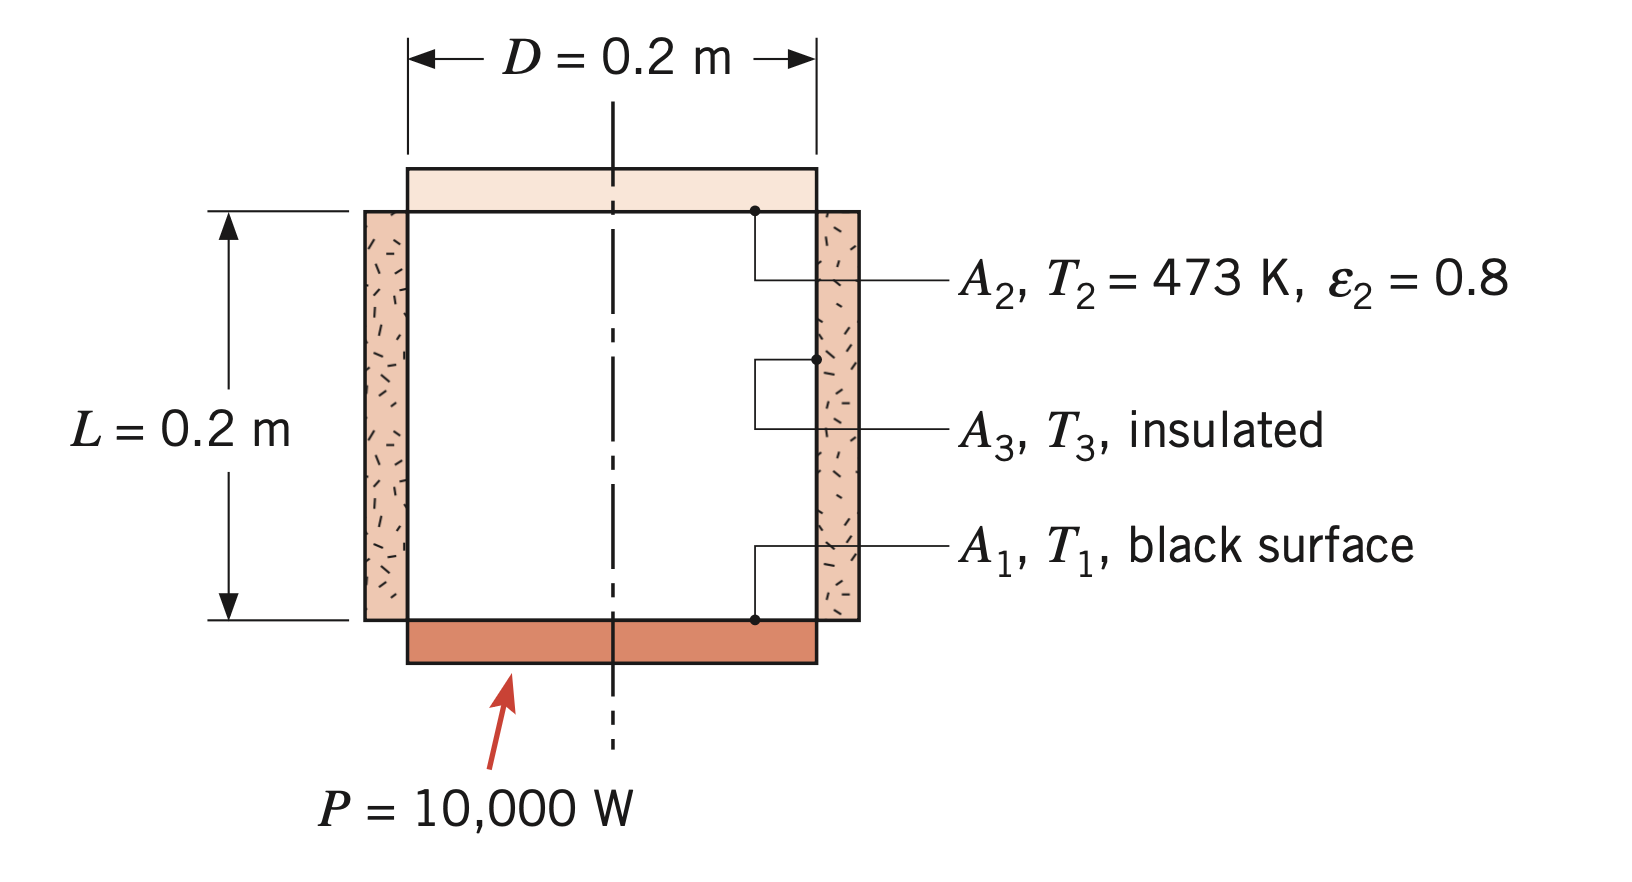
\includegraphics[width=0.75\linewidth]{./radiation_image.png}
    \end{figure}

    \item You are running an experiment using naphthalene in a wind tunnel.
        The (relatively wide) naphthalene surface \SI{10}{\centi\meter} is placed a meter downstream of a trip wire and is flush with the wind tunnel wall.
        If the wind tunnel velocity is \SI{10}{\meter\per\second}, what is the change in height of the naphthalene surface?
        \begin{enumerate}
            \item Find the surface temperature of the naphthalene.
                Do you expect heat transfer to be important?
                Plot the 
                \begin{enumerate}
                    \item ratio of the heat transfer coefficient and the heat transfer coefficient at low rates of mass transfer as a function of the naphthalene evaporation rate, and
                    \item ratio of the heat transfer and the heat transfer at low rates of mass transfer as a function of the naphthalene evaporation rate.
                \end{enumerate}
            \item Find the saturation pressure of the naphthalene concentration just above the surface.
                Will the properties of air need to be adjusted for the presence of naphthalene? 
            \item Find the blowing factor.
                Will a correction to the mass transfer coefficient need to be made for high mass transfer rates?
                Plot the ratio of the mass transfer coefficient and the mass transfer coefficient at low rates of mass transfer as a function of the blowing ratio.
            \item Finally, plot the sublimed depth of the naphthalene along the surface in the streamwise direciton.
        \end{enumerate}

    \item Dry ice (solid $\mathrm{C} \mathrm{O}_2$) is used to cool medical supplied transported by a small plane to a remote village in Alaska.
        A roughly spherical chunk of dry ice, \SI{5}{\centi\meter} in diameter, falls from the plane through air at \SI{5}{\celsius}.
        It reaches a terminal velocity of \SI{40}{\meter\per\second}.
        What are the temperature and sublimation rate of the dry ice, assuming steady conditions?
        The latent heat of sublimation is about \SI{590}{\kilo\joule\per\kilogram} and $\mathrm{log}_{10} \left( p_v  \right) = 6.81228 - 1301.679 / \left( T - 3.494 \right)$, where pressure is in bars and temperture is in Kelvin.
        The surface temperature will be well below the solid-vapor equilibrium temperature of $\mathrm{C} \mathrm{O}_2$ at 1 atm, which is \SI{-78.5}{\celsius}.
        Use this correlation for forced convection of a sphere at room temperature

        \begin{equation*}
                \overline{\mathit{Nu}}_D = 2 + 0.493 \mathit{Re}_D^{1/2} + 0.0011 \mathit{Re}_D
        \end{equation*}

        for $7800 \leq \mathit{Re}_D \leq \num{2.9e5}$.
        Neglect heat conduction into the ice.
\end{enumerate}

\end{document}
